\setcounter{chapter}{1}
\chapter{Méthodes Physiques d'analyse}
\section{Spectroscopie UV, Visible}
\subsection{Rappels}
On appelle lumière visible les ondes électromagnétiques dont la longueur d'onde $\lambda$ est comprise entre \trou{ 400 nm et 800 nm.}

\subsection{Solution colorée et absorbance}

Certaines espèces en solutions sont colorées (l'ion permanganate, le diiode, etc). Cette couleur est due à l'absorption de certaines radiations. Le \trou{spectre d'aborption} d'une espèce montre quelles sont les radiations absorbées.

\begin{figure*}[htp!]
	\begin{center}
		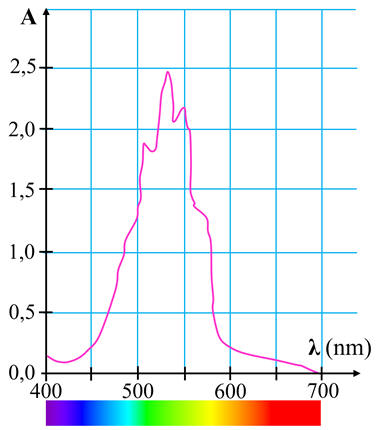
\includegraphics[scale=.4]{figures/spectre_permanganate_2}
		\caption{Spectre d'absorption de l'ion $MnO^{4-}$}
	\end{center}
\end{figure*}

On peut prédire la couleur de la solution en prenant la couleur complémentaire de la couleur la plus absorbée.

Par exemple, l'ion permanganate absorbe dans le jaune-vert. La couleur de la solution de permanganate est violette.


\begin{figure*}[htp!]
	\begin{center}
		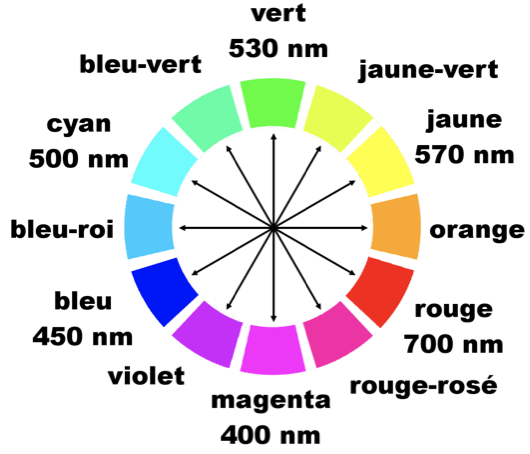
\includegraphics[scale=.6]{figures/cercle_chromatique}
		\caption{Couleurs complémentaires}
	\end{center}
\end{figure*}



\subsection{Spectrophotomètre et Absorbance}
Un spectrophotomètre mesure l'absorbance A d'une solution.

\blocrouge{Définition}{L'absorbance est notée $A$  et qualifie la capacité d'une solution à absorber la lumière (pour une longueur d'onde $\lambda$ fixée). A est un nombre sans unité. }

\paragraph*{Interprétation}

Plus A est grande, plus la solution absorbe et sa coloration est \trou{foncée}.

\blocrouge{Loi de Beer-Lambert}{Pour une solution de concentration $c$ l'absorbance A vaut $$A=k\times c$$ avec $k$ une constante qui dé pend du soluté et de l'épaisseur $\ell$ de la cuve.
De manière plus détaillée, on a $k=\epsilon\times \ell$ avec $\epsilon$ le coefficient d'extinction molaire. 

On peut donc écrire $$A=\trou{ \epsilon\times \ell\times c}$$
}


\etiquetterouge{Important} La loi de Beer-Lambert modélise le relation entre A et c. Ce modèle est bien vérifiée lorsque la concentration est inférieure  à $10^{-2}$ mol/L.

\etiquette{Compléments} L'absorbance se calcule partir de l'intensité lumineuse incidente $I_0$ et l'intensité lumineuse transmise $I_1$ selon $$A = \log{\frac{I_1}{I_0}}$$
\begin{figure*}[htp!]
	\begin{center}
		\includegraphics{figures/fig6}
		\caption{Intensité lumineuse transmise et absorbance}
	\end{center}
\end{figure*}

\subsection{Principe du dosage par étalonnage}

\etiquette{But} On souhaite connaître la concentration d'une solution colorée.

\blocgris{Méthode} 
{
\begin{itemize}
\item Préparer des solutions étalons de concentrations connues par dilution d'une solution contenant l'espèce à doser.
\item Pour chaque solution mesurer l'absorbance.
\item Tracer la droite d'étalonnage, l'absorbance en fonction de la concentration.
\item Mesurer l'absorbance de la solution de concentration inconnue.
\item Utiliser la droite d'étalonnage pour en déduire la concentration cherchée.
\end{itemize}
}

\etiquetterouge{Exercices} 4 p 40 et 17 p 43.
\section{Spectroscopie infrarouge (IR)}
\subsection{Principe}

On constate que certaines radiations électromagnétiques dont les longueurs d'ondes sont dans le domaine de l'infrarouge ($\lambda >800$ nm) sont aborbées par les liaisons chimiques contenues dans une molécule. La valeur de la longueur d'onde absorbée peut être mise en relation avec un type particulier de liaison chimique.

Ces informations se retrouvent sur le spectre IR d'une molécule.

\subsection{Analyse d'un spectre}

Un spectre IR se présente comme ceci :\\
\begin{center}
\includegraphics[scale=0.5]{figures/pentan-2-ol_IR}
\end{center}
En ordonnée, la transmittance, exprimée en pourcentage. 100\% signifie que la radiation n'est pas du tout absorbée, tout est transmis.\\
En abscisse, \trou{le nombre d'onde, noté $\sigma$ et exprimé en $\SI{}{\per\centi\meter}$. Le nombre d'onde est l'inverse de la longueur d'onde, c'est à dire que $\sigma = \dfrac{1}{\lambda}$}\\
Dans le spectre, on observe des bandes d'absorption. Ces bandes correspondent à des liaisons bien particulières, ce qui permet d'identifier dans la molécule des groupes caractéristiques.\\
Pour cela, nous utilisons des tables de référence (cf p 35 de votre livre)

\subsection{Application}
\etiquette{Activité documentaire 2 p 32}
\etiquetterouge{Exercice} 23 p 46

\section{La conductimétrie}
La conductimétrie est basée sur l'étude de la capacité d'une solution à conduire le courant électrique. On ne pourra donc faire une étude conductimétrique qu'avec des solutions électrolytiques, c'est à dire des solutions comportant des ions.
\subsection{La conductance}
Une cellule conductimétrique est constituée de 2 plaques métalliques planes et parallèles de même surface S, distantes de $\ell$, les électrodes.\\
Un conductimètre mesure la résistance de la solution qui se trouve contenue entre les deux plaques.

	\begin{figure*}
	\begin{center}
		\includegraphics[scale=.5]{figures/conductimetre}
	\end{center}
	\end{figure*}

\blocrouge{Définition}{
La conductance est définie comme étant l'inverse de la résistance, c'est à dire : \\
\trou{$G=\dfrac{I}{U}$ avec G en siemens (S) ; I en ampères (A), et U en volts (V)}
}

La résistance est une grandeur représentative de la capacité de la solution à \trou{s'opposer }au passage du courant électrique.\\
La conductance est une grandeur représentative de la capacité de la solution à \trou{conduire }le courant électrique.
\subsection{La conductivité}
La conductance est proportionnelle à l'aire S des électrodes et inversement proportionnelle à la distance $\ell$ les séparant.\\
On a donc $G=\trou{\sigma \dfrac{S}{\ell}}$ ou $\sigma$ est une grandeur notée la conductivité de la solution.

\blocrouge{Définition de la conductivité}{
On a alors $\sigma = \trou{G\dfrac{\ell}{S}}$\\
Avec $\sigma$ \trou{la conductivité en $\SI{}{\siemens\per\meter}$}\\
G \trou{la conductance en S}\\
$\ell$ \trou{la distance entre les plaques en m}\\
S \trou{la surface immergée des électrodes.}
}

Pour une même cellule conductimétrique, la conductivité dépend donc uniquement des caractéristiques de la solution, température, nature et concentration des ions.

\subsection{La loi de Kohlrausch}
Tous les ions n'ont pas la même capacité à conduire le courant électrique. \\
L'influence de la nature de l'ion est caractérisée par la conductivité molaire ionique $\lambda$. %Elle s'exprime en $\SI{}{\siemens\meter\squared\per\mole}$

\blocrouge{Loi de Kolhrausch}{
$\sigma =\trou{\sum\limits_{i=1}^n \lambda_i[X_i]}$\\
Avec $\sigma$ en \trou{$\SI{}{\siemens\per\meter}$}\\
$\lambda$ en \trou{$\SI{}{\siemens\meter\squared\per\mole}$}\\
et [X] en \trou{$\SI{}{\mole\per\meter\cubed}$}\\
\underline{Remarque :} Cette loi n'est valable que pour les solutions de concentration peu élevées (inférieures à $\SI{0,01}{\mole\per\liter}$, c'est à dire $\SI{10}{\mole\per\meter\cubed}$).\\

}
%\vspace{1cm}

\etiquette{Application}
Soit une solution de nitrate d'argent $(Ag^+ + NO_3^-)$ de concentration $\SI{1,0e-2}{\mole\per\liter}$.\\
$Ag^+ = \SI{6,19}{mS.m^2.mol^{-1}} $;
$NO_3^-= \SI{7,14}{mS.m^2.mol^{-1}}$
\begin{enumerate}
\item A partir de la loi de Kolhrausch,  exprimer la conductivité de la solution en fonction des conductivités molaires ioniques des ions présents.
\item Appliquer cette relation pour trouver la valeur de la conductivité de la solution.
\end{enumerate}
\vspace{8cm}

\subsection{Détermination de la concentration d'une solution à partir de sa conductivité}
On obtient une solution, de concentration inconnue c, par dissolution dans l'eau de nitrate de nickel de formule $Ni(NO_3)_2(s)$\\
 On mesure sa conductivité, et l'on trouve $\sigma=\SI{5,00e-2}{\siemens\per\meter}$.\\
 
\begin{enumerate}
\item Ecrire l'équation de dissolution du nitrate de nickel dans l'eau.\\
\trou{$Ni(NO_3)_2(s) \longrightarrow Ni^{2+}(aq) + 2NO_3^-(aq)$}
\item Exprimer, en fonction de c, les concentrations des ions en solution.\\
\trou{$[Ni^{2+}]=c$ et $[NO_3^-]=2c$}
\item Appliquer la loi de Kolhrausch puis exprimer la conductivité dela solution $\sigma$ en fonction des conductivités molaires ioniques des ions présents en solution et de c.\\
\trou{$\sigma=\lambda_{Ni^{2+}}[Ni^{2+}]+\lambda_{NO_3^-}[NO_3^-]$\\
$\sigma = (\lambda_{Ni^{2+}}+2\lambda_{NO_3^-})\times c$\\}
\paragraph*{Remarque :}
\trou{On constate que la conductivité est proportionnelle a la concentration en soluté apporté. $\sigma = k \times c$.}
\item En déduire la valeur de c.\\
\trou{Donc $c=\dfrac{\sigma}{\lambda_{Ni^{2+}}+2\lambda_{NO_3^-}}=\dfrac{\num{5,00e-2}}{\num{10,8e-3}+2\times \num{7,1e-3}}=\SI{2,00}{\mole\per\meter\cubed}=\SI{2,00e-3}{\mole\per\liter}$}
\end{enumerate}


\subsection{Dosage conductimétrique par étalonnage}
\blocgris{Principe d'un dosage par étalonnage}{
Les différentes étapes du dosage par étalonnage conductimétrique: 
\begin{itemize}
\item Préparer des solutions étalons de concentrations connues par dilution d'une solution contenant l'espèce à doser.
\item Pour chaque solution, mesurer la conductance ou la conductivité.
\item Tracer la courbe d'étalonnage : la conductance ou la conductivité en fonction de la concentration.
\item Mesurer la conductance ou la conductivité de la solution de concentration inconnue.
\item Utiliser la droite d'étalonnage pour en déduire la concentration recherchée.
\end{itemize}
}


\etiquetterouge{Important}  La loi de Kolhrausch suppose que la solution ionique est suffisamment diluée ($c<\SI{10e-2}{\mole\per\liter}$) 


\etiquetterouge{Exercices} 6, 7, 14 p 40-42 +  Préparation ECE p 47

\section{Les gaz parfaits}

\subsection{Equation d'état des gaz parfaits}
A l'échelle microscopique, un gaz est modélisé par un ensemble d'entités en mouvement désordonné. Si les interactions entre les entités sont négligeables, un gaz est dit <<parfait>>.  C'est le cas de tous les gaz à basse pression.\\
\blocrouge{Equation d'état des gaz parfaits}{
\trou{$P\times V=n\times R \times T$}\\
Avec P \trou{la pression en Pascal (Pa)}\\
V \trou{le volume en $\SI{}{\meter\cubed}$}\\
n \trou{la quantité de matière en mole (mol)}\\
T \trou{la température en Kelvin (K)}\\
R \trou{la constante des gaz parfait }: $R=\trou{\SI{8,314}{\pascal\meter\cubed\per\mole\per\kelvin}}$
}

On peut donc, à partir de cette équation, calculer une quantité de matière de gaz.

\etiquette{Application}
Sous une pression de $\SI{1,20e5}{\pascal}$, et à une température de $\SI{22}{\celsius}$, un échantillon de gaz supposé parfait occupe un volume égal à $\SI{0,31}{\liter}$. Calculer la quantité de matière correspondante.\\
\trou{$n=\dfrac{PV}{RT}=\SI{1,5e-2}{\mole}$}
\subsection{Volume molaire}
\blocrouge{Définition}{
Le volume molaire des gaz $V_m$ est \trou{le volume occupé par une mole de gaz pour une température et une pression données. Il ne dépend pas de la nature du gaz.\\
on a : $n=\dfrac{V}{V_m}$\\
Avec n la quantité de matière en mol\\
V le volume en L\\
$V_m$ le volume molaire en $\si{\liter\per\mole}$}
}

On a, d'après l'équation d'état des gaz parfaits, $n=\trou{\dfrac{PV}{RT}}$.\\
Or, n est aussi égal à $n=\trou{\dfrac{V}{V_m}}$\\
On en déduit que $V_m=\trou{\dfrac{RT}{P}}$. On retrouve bien que c'est une constante pour une températures et une pression données.


\etiquette{Application}
Calculer le volume molaire à pression standard $\SI{1,01e5}{\pascal}$ et à une température de $\SI{25}{\celsius}$.
\vspace{3cm}

\etiquette{Exercices} 19, 20 et 24 p 44

\etiquetterouge{Synthèse} Résume ici l'essentiel de ce chapitre: ce qu'il faut savoir par coeur et les techniques à connaître.



